%Dies ist die Hauptseite des Dokumentes. Es werden u. a. alle Kapitel,
%Einstellung im Header eingebunden.
%Veränderungen müssen in folgenden Dateien vorgenommen werden:
      %- Layout.tex
      %- newComments.tex
      %- Titelseite
      %- Versionsübersicht
      %- einzelne Kapitel (evtl. erweitern)


% Definition von globalen Parametern, die derzeit auf der Titelseite und in der
% Kopfzeile verwendet werden. Der in <> gesetzte Text ist zu verändern.

\newcommand{\praktikumTitel}{Ingenieursmäßige Konstruktion, Simulation und Visualisierung von Achterbahnen }
\newcommand{\projektTitel}{Achterbahnsimulator}


%Hier sind alle Einstellungen enthalten, die sich auf das Seiten- und
%Dokumentenlayout beziehen

\documentclass[
  11pt,                % Schriftgröße
  DIV12,
  german,              % für Umlaute, Silbentrennung etc.
  oneside,             % einseitiges Dokument
  titlepage,           % es wird eine Titelseite verwendet
  halfparskip,         % Abstand zwischen Absätzen (halbe Zeile)
  normalheadings,      % Größe der Überschriften verkleinern
  tablecaptionabove,   % Beschriftung von Tabellen unterhalb ausgeben
  final                % Status des Dokuments (final/draft)
]{scrreprt}            %


%------Ändern von Schriftschnitten - (Muss ganz am Anfang stehen !) ------------
\usepackage{fix-cm}

%------Umlaute -----------------------------------------------------------------
%   Umlaute/Sonderzeichen wie äüöß können direkt im Quelltext verwenden werden.
%    Erlaubt automatische Trennung von Worten mit Umlauten.
\usepackage[T1]{fontenc}
\usepackage[utf8]{inputenc}

%------Anpassung der Landessprache----------------------------------------------
\usepackage{ngerman}

%------Einfache Definition der Zeilenabstände und Seitenränder------------------
\usepackage{geometry}
\usepackage{setspace}

%------Schriftgrößenanpassung von einzelnen Textpassagen------------------------
\usepackage{relsize}

%------Trennlinien in Kopf- und Fusszeile
\usepackage[headsepline, footsepline, ilines]{scrpage2}

%------Grafiken-----------------------------------------------------------------
\usepackage{graphicx}

%------Packet zum Sperren, Unterstreichen und Hervorheben von Texten------------
\usepackage{soul}

%------ergänzende Schriftart----------------------------------------------------
\usepackage{helvet}

%------Lange Tabellen-----------------------------------------------------------
\usepackage{longtable}
\usepackage{array}
\usepackage{ragged2e}
\usepackage{lscape}

%------PDF-Optionen-------------------------------------------------------------
\usepackage[
  bookmarks,
  bookmarksopen=true,
  colorlinks=true,
  linkcolor=black,        % einfache interne Verknüpfungen
  anchorcolor=black,      % Ankertext
  citecolor=black,        % Verweise auf Literaturverzeichniseinträge im Text
  filecolor=black,        % Verknüpfungen, die lokale Dateien öffnen
  menucolor=black,        % Acrobat-Menüpunkte
  urlcolor=black,         % Farbe für URL-Links
  backref,                % Zurücktext nach jedem Bibliografie-Eintrag als
                          % Liste von Überschriftsnummern
  pagebackref,            % Zurücktext nach jedem Bibliografie-Eintrag als
                          % Liste von Seitenzahlen
  plainpages=false,       % zur korrekten Erstellung der Bookmarks
  pdfpagelabels,          % zur korrekten Erstellung der Bookmarks
  hypertexnames=false,    % zur korrekten Erstellung der Bookmarks
  linktocpage             % Seitenzahlen anstatt Text im Inhaltsverzeichnis
                          % verlinken
  ]{hyperref}



      % enthält eingebundene Packete

%------Seitenränder-------------------------------------------------------------
\geometry{verbose,                     % zeigt die eingestellten Parameter beim
                                       % Latexlauf an
      paper=a4paper,                   % Papierformat
      top=25mm,                        % Rand oben
      left=25mm,                       % Rand links
      right=25mm,                      % Rand rechts
      bottom=45mm,                     % Rand unten
      pdftex                           % schreibt das Papierformat in die
                                       % Ausgabe damit Ausgabeprogramm
                                       % Papiergröße erkennt
  }

%Seitenlayout
\onehalfspace        % 1,5-facher Abstand

%------Kopf- und Fußzeilen -----------------------------------------------------
\pagestyle{scrheadings}

%------Kopf- und Fußzeile auch auf Kapitelanfangsseiten ------------------------
\renewcommand*{\chapterpagestyle}{scrheadings}

%------Schriftform der Kopfzeile -----------------------------------------------
\renewcommand{\headfont}{\normalfont}

%------Kopfzeile----------------------------------------------------------------
\setlength{\headheight}{21mm}        % Höhe der Kopfzeile
\ihead{\large{\textsc{\praktikumTitel}}\\    % Text in der linken Box
       \small{\projektTitel}}
\chead{}                             % Text in der mittleren Box

%----Fusszeile
\cfoot{}                             % Text in mittlerer Box
\ofoot{\pagemark}                    % Seitenzahl in rechter Box

          % Diese Datei enthält alle
                                          % Layouteinstellungen

%------Beginn des Gesamtdokumentes----------------------------------------------
\begin{document}

%------Eingebundene Seiten, Verzeichnisse bzw. Kapitel--------------------------
% Dies ist die Titelseite des Pflichtenhefts.
% Die in "<...>" sind zu ersetzen
% Die Ausgabe darf 1 Seite nicht überschreiten, also ggf. Abstände anpassen
% Die Angabe in [...] gibt den Abstand nach der entsprechenden Zeile an.


%----Stil dieser Seite----------------------------------------------------------
\thispagestyle{plain}      % Kopfzeile bleibt leer

%----Beginn der Titelseite------------------------------------------------------
\begin{titlepage}

%----zentrierte Ausrichtung über die gesamte Seite----------------------------
\begin{center}

%----Titel des Praktikum (\praktikumTitel in newComments zu verändern)--------
{\relsize{4}{\textbf{\textsc{\praktikumTitel}}}}\\[5ex]

%----Titel des Teilprojektes (\projektTitel in newComments verändern)---------
{\relsize{3}{\textbf{\textsc{\projektTitel}}}}\\[5ex]

Software-Entwicklungspraktikum (SEP)\\
Sommersemester 2011\\[6ex]

{\relsize{3}\so{\textbf{Pflichtenheft}}}\\[5ex]

%----eingebundenes Logo der TU--------------------------------------------------

\includegraphics[scale=0.8]{bilder/carolo.jpg}\\[5ex]

%----Daten des Auftraggebers
Auftraggeber\\
Technische Universität Braunschweig\\
Institut für Wissenschaftliches Rechnen\\
Prof. Hermann G. Matthies, PhD\\
<Straße und Hausnummer>\\
D-38092 Braunschweig\\[2ex]
Betreuer: Elmar Zander\\[5ex]

% ----Tabelle der Praktikumsteilnehmer------------------------------------------
Auftragnehmer: <überzählige Zeilen löschen>\\

\begin{tabular}{l<{\hspace{20mm}} l<{\hspace{30mm}}}\\
  Name                   &   E-Mail-Adresse\\      % Zeilenüberschift

  \hline                    % Linie unterhalb der Zeilenüberschrift

  %----Nachfolgend alle Namen und E-Mail-Adressen der Teilnehmer einfügen
  Matthias Überheide> &  m.ueberheide@tu-bs.de\\
  Christian Mangelsdorf &  ch.mangelsdorf@googlemail.com\\
	Daniel Bahn & danielbahn@arcor.de\\
	Simon Hahne & MrSimWob@aol.com\\
	Robin Hofmann & hofmann.robin@web.de\\
	Marco Melzer & marco.melzer@tu-braunschweig.de\\
	Konstantin Birker & k.birker@tu-braunscheig.de\\

\end{tabular}\\[2ex]

Braunschweig, \today

\end{center}
\end{titlepage}
                      % Titelseite

%Diese Datei dient der Versionskontrolle. Sie ist vollständig zu bearbeiten.

%----Überschrift------------------------------------------------------------
{\relsize{2}\textbf{Versionsübersicht}}\\[2ex]

%----Start der Tabelle------------------------------------------------------
\begin{longtable}{|m{1.78cm}|m{1.59cm}|m{2.86cm}|m{1.9cm}|m{5.25cm}|}

  \hline                                              % Linie oberhalb

  %----Spaltenüberschriften------------------------------------------------
  \textbf{Version}  &    \textbf{Datum}  &    \textbf{Autor}  &
  \textbf{Status}   &    \textbf{Kommentar}       \\  %Spaltenüberschrift
  \hline                                              % Gitterlinie

  %----die nachfolgeden beiden Zeilen so oft wiederholen und die ... mit den
  %    entsprechenden Daten zu füllen wie erforderlich
  0.1&02.05.2011&Christian Mangelsdorf&in Bearbeitung&Initialisierung\\
  \hline
  0.2&04.05.2011&Simon Hahne, Robin Hoffman, Christian Mangelsdorf&in Bearbeitung&Komponentenspezifiktion\\
  \hline
  0.3&06.05.2011&Matthias Überheide&in Bearbeitung&Vorbereitung Funktionsanalyse\\
  \hline
  0.4&08.05.2011&Matthias Überheide, Daniel Bahn, Konstantin Birker, Robin Hoffman, Simon Hahne, Christian Mangelsdorf&in Bearbeitung&Sequenzdiagramme und Statcharts\\
  \hline
  0.5&09.05.2011&Matthias Überheide, Daniel Bahn, Robin Hoffman, Simon Hahne, Christian Mangelsdorf&in Bearbeitung&Änderungen gemäß Besprechung\\
  \hline
  0.6&10.05.2011&Matthias Überheide, Christian Mangelsdorf&in Bearbeitung&Schnittstellenspezifikation\\
  \hline
  0.7&11.05.2011&Matthias Überheide, Daniel Bahn, Konstantin Birker, Robin Hoffman, Simon Hahne, Christian Mangelsdorf, Marco Melzzer&abgenommen&Korrekturen\\
  \hline
  %...    &    ...    &    ...    &    ...    &    ...\\       % Eintrag in Zeile
  \hline                                              % Gitterlinie unten

%----Ende der Tabelle------------------------------------------------------
\end{longtable}

%Status: "`in Bearbeitung"' oder "`abgenommen"'
%Kommentar: hier eintragen, was geändert bzw. ergänzt wurde


%Hinweis zum Template:
%Dieses Template enthält Hinweise, die alle kursiv geschrieben sind. Alles
%Kursivgeschriebene ist selbstverständlich bei Abgabe zu entfernen sind.
%Angaben in <\ldots> sind mit dem entsprechendem Text zu füllen.  Überzählige
%Kapitel, d. h. Kapitel, die nicht bearbeitet werden müssen, da sie nicht der
%Aufgabenstellung entsprechen, bitte entfernen.

%Aufgabe des Grobentwurfs: Aufgabe dieses Dokumentes ist es, die Architektur des
%Systems zu beschreiben und die daraus resultierenden Pakete durch die
%Definition von Schnittstellen zu Komponenten auszubauen.
       % Versionsübersicht

\tableofcontents                          % Inhaltsverzeichnis wird automatisch
                                          % generiert
\listoffigures                            % ebenso das Abbildungsverzeichnis

%----Kapitel des Feinentwurfs, die mit Inhalt zu füllen sind--------------------
% Kapitel 1
% Die Unterkapitel können auch in separaten Dateien stehen,
% die dann mit dem \include-Befehl eingebunden werden.
%-------------------------------------------------------------------------------

\chapter{Einleitung}
%Hier Einleitungstext einfügen, dabei die Formatierungen selber erstellen
%Hier ist die Arbeitsweise des Systems anhand von State-Charts darzustellen und kurz zu erläutern.

Die Anwendung ist ein Werkzeug zur physikalischen Simulation und 3D-Visualisierung von Achterbahnfahrten.
Der Benutzer wählt dazu eine Datei mit der Spezifikation des Streckenverlaufes aus. Die Anwendung erstellt 
daraus ein virtuelles Modell der Achterbahn und simuliert physikalisch korrekt die Bewegung des Wagens mit
der Zeit. In den folgenden Abschnitten wird Arbeitsweise des Simulators detailiert.

\section{Projektdetails}
Die Funktionalität der Anwendung gliedert sich in mehrere zusammenhängende Teilbereiche. Jeder dieser
Bereiche bündelt eine Reihe der Anforderungen, die im Pflichtenheft spezifiziert worden sind.

\subsection{Benutzeroberfläche}
Über die Benutzeroberfläche (GUI) werden dem Anwender alle vorhandenen Funktionen zugänglich gemacht.
Nach dem Programmstart befindet sich der Anwender in einem Initialzustand: Die Felder des 2D-Modells
und der 3D-Darstellung befinden sich in einem Blanko-Zustand und die physikalischen Parameter sind
auf die Standardwerte gesetzt. Der nächte Schritt ist die Auswahl einer Datei mit den Konstruktionsdaten
über ein Dateimenü. Nach dem Einlesen der Datei zeigt die Anwendung zunächst eine zweidimensionale 
Vorschau der Achterbahn an. Zu diesem Zeitpunkt können über ein Optionen-Menü verschiedene Anpassungen 
an den Grafikeinstellungen und den physikalischen Parameter vorgenommen werden. 
Aus der Vorschau heraus kann die Simulation gestartet werden. Ab diesem Zeitpunkt wird das Feld für 
die 3D-Darstellung befüllt. Auf Wunsch kann die 3D-Darstellung auf Bildschirmgröße
maximiert werden. Während der laufenden Simulation können die Grafikeinstellungen, nicht jedoch
die physikalischen Simulationsparameter angepasst werden. Wird die Simulation gestoppt, kehrt die Anwendung
wieder in die Vorschau zurück. Durch Schließen der Achterbahndatei gelangt der Benutzer wieder in den 
Initialzustand.

\begin{figure}
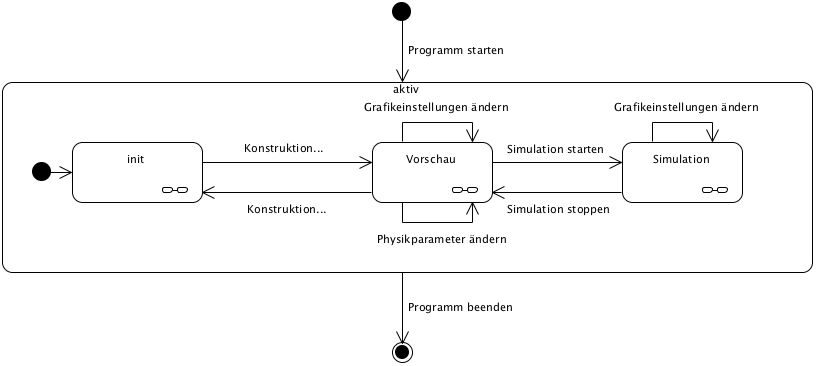
\includegraphics[width=\linewidth]{bilder/StateChart_GUI}
\caption{Statechart für die \textit{Benutzeroberfläche}}
\end{figure}

\subsection{Simulator}
Der Simulator ist das Kernstück der Anwendung und repräsentiert das Zusammenspiel aus physikalischen Berechnungen
und grafischer Darstellung der Achterbahnfahrt. Die Zustandswechsel des Simulators verlaufen synchron mit 
denen der Benutzeroberfläche. Nach dem Starten des Programms befindet sich der Simulator in einem Initialzustand,
der noch keine Simulation repräsentiert. Durch das Befüllen mit der Spezifikation der Achterbahn wird
eine Simulation instanziert und zur Vorschau gebracht. Mit dem Start der Simulation werden in diskreten Zeitschritten
die aktualisierten physikalischen Daten eingelesen und zur Veränderung der Kameraposition verwendet. Durch das
Stoppen der Simulation kehrt auch der Simulator wieder in die Vorschau zurück.

\subsection{3D-Anzeige}
Die 3D-Anzeige dient zur Visualisierung der Achterbahnfahrt, also zur Darstellung der Bahn als 3D-Modell aus
einer vorgegebenen Kameraperspektive. Vor der Bereitstellung eines konkreten Achterbahnmodells befindet sich
die Anzeige in einem Initialzustand, in welchem es in Ermangelung von Daten nicht möglich eine Szene darzustellen. 

\begin{figure}
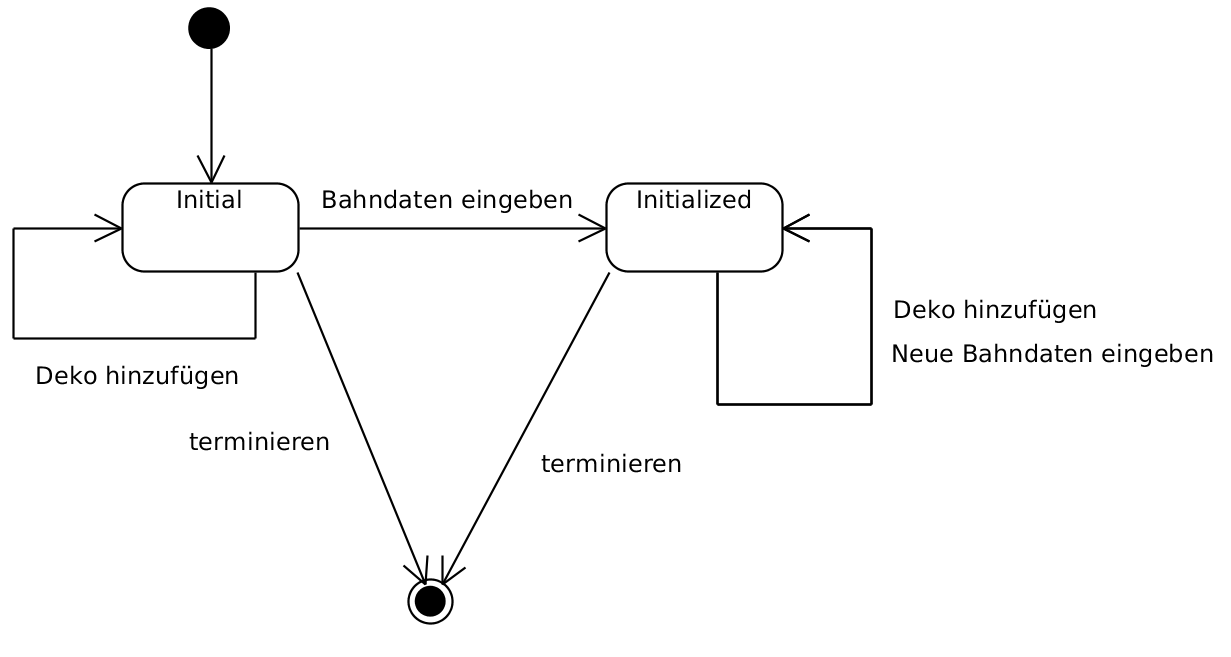
\includegraphics[width=\linewidth]{bilder/statechart_3dgraphics}
\caption{Statechart für die \textit{3D-Anzeige}}
\end{figure}

Durch Übergabe der Bahndaten kann die 3D-Anzeige die Achterbahn und deren Umgebung für die Anzeige vorberechnen.
Aber erst nach dem Start der Simulation, werden regelmäßig Bilder berechnet und angezeigt. Aus Sicht der 3D-Anzeige
können nach der Beladung jederzeit Änderungen wie Einfügen von Dekoration oder Anpassen der grafischen Einstellungen
vorgenommen werden, ohne das eine Zustandsänderung erforderlich wäre. Allerdings müssen innerhalb des Render-Vorgangs
eines einzelnen Bildes die Einstellungen unverändert bleiben, damit eine saubere Kommunikation mit dem 3D-Hardwarekontext
gewahrt bleibt.

\subsection{Physik und Mathematik}

Die physikalischen Berechnungen des Achterbahnsimulators folgen den Gesetzen der Newtonschen Mechanik für die Bewegung
eines Massenpunktes auf einer vorgegebenen Bahn im Gravitationsfeld der Erde. Berechnet wird die Bahnkurve als Lösung
einer gewöhnlichen Differentialgleichung mit vorgegebenen Anfangswerten. Die Lösung erfolgt nach einem numerischen
Verfahren, welches über die Zeit integriert.

Entsprechend wird der Zustand des Systems nach der Initialisierung mit den Bahndaten und den Anfangswerten von Zeitpunkt
zur Zeitpunkt weiterentwickelt, bis die Simulation (z.B. über Programmende) beendt wird.

Für die Berechnung der Bahnkurven kommen eine Reihe von Hilfsmethoden zum Einsatz. Diese Routinen sind zustandslos und
besitzen keinen eigenen Lebenszyklus.

\begin{figure}
\includegraphics[width=\linewidth]{bilder/statechart_physics}
\caption{Statechart für die \textit{Physik}}
\end{figure}
               % Kapitel 1
% Kapitel 2 mit den entsprechenden Unterkapiteln
% Die Unterkapitel können auch in separaten Dateien stehen,
% die dann mit dem \include-Befehl eingebunden werden.
%----------------------------------------------------------------------------

\chapter{Testplan}

Der Testplan ist das zentrale Dokument der Qualitätssicherung und wird daher
frühzeitig erstellt. Hier wird Umfang und Vorgehensweise der Qualitätssicherung
beschrieben. Außerdem werden Testgegenstände und deren zu testenden
Eigenschaften bzw. Funktionen identifiziert. Ferner werden die
durchzuführenden Maßnahmen und die dafür verantwortlichen Personen definiert.
Falls erforderlich sollte hier auch auf allgemeine Risiken eingegangen werden.

\section{Zu testende Komponenten}
Der Achterbahnsimulator ist eine Einzelplatzanwendung. Das fertige Produkt wird als monolitisches System abgenommen und ist deswegen im strengen Sinne keine verteile Anwendung. Da jedoch zu den Anforderungen an den Simulator das Einlesen der Achterbahndaten aus dem Editor zählt, muss dieses Zusammenspiel geprüft werden.

Der Achterbahnsimulator setzt sich gemäß Entwurf aus verschiedenen Komponenten zusammen, deren Aufteilung bei der Implementierung zur Beibehaltung der Konhärenz inenrhalb der Komponenten und Vermeidung von zwischen den Komponenten beizubehalten war.
Entsprechend können diese Komponenten getrennt geprüft werden. 

Da die Software eine 3D-Anzeige beeinhaltet ist es vor dem Test sicherzustellen, dass die Grafikkarte entsprechend inklusive 3D-Beschleunigung eingerichtet ist.
Die Software kann online (im Repository) oder lokal auf Festplatte oder CD vorliegen. In jedem Fall ist dafür Sorge zu tragen, dass die Software die Möglichkeit hat in dem lokalen Pfad Dateien anzulegen.

\section{Zu testende Funktionen}
% Dieser Punkt beinhaltet alle Eigenschaften bzw. Funktionen und deren
% Kombinationen, die zu testen sind.
% 
% Sämtliche Funktionalitäten, die getestet werden sollen, werden hier aufgeführt.
% Dabei sind auf die vorangegangenen Dokumentationen zu referenzieren
% (Pflichtenheft, Grob- und Fein-entwurf) und die dortigen Funktions-IDs zu
% verwenden!\\ Beispiel: /F100/ : Benutzer Login
Im folgenden findet sich eine Liste über die Funktionen des Programms die zu testen sind. 

/F100/ : Spezifikation einlesen\\
\\
/F200/ : Starten/Stoppen der Simulation\\
\\
/F300/ : Pausieren der Simulation\\
\\
/F500/ : Einstellungen ändern\\
\\
/F520/ : Simulationsparameter ändern\\
\\
/F530/ : Grafische Einstellungen ändern\\
\\
/F531/ : Neuanordnung (Interface)\\
\\
/F532/ : Ein-/Ausblenden von Beschleunigungsdaten\\
\\
/F533o/ : Kameraperspektive ändern\\
\\
/F1000/ : Warnung vor zu hoher Beschleunigung\\
\\
/F1100/ : Erkennung von Veränderungen an der Ursprungsdatei



HIER ERSTMLA NUR DIE MUSS KRITERIEN... NOCH NICHT FERTIG!!!

\section{Nicht zu testende Funktionen}
(optional; auszufüllen, falls es Funktionen gibt, die nicht getestet werden
sollen)\\

Hier werden alle Eigenschaften bzw. Funktionen und Funktionskombinationen
aufgelistet, die nicht getestet werden.
\textbf{ Es sollte begründet werden, warum diese nicht getestet werden.} Es
versteht sich von selber, dass alle Muss-Funktionalitäten des Pflichtenheftes
(Abschnitt 1.1) getestet werden müssen.

\section{Vorgehen}

Während sich für den mathematisch-physikalischen Kern der Anwendung eine Prüfung mit automatisierten Tests umsetzen lässt, müssen diese für die visuellen Komponenten der GUI und 3D-Grafik weitestgehend händische vorgenommen werden.

Für die Durchführung der JUnit-Testfälle wurde ein \textbf{ant}-Task in der \textbf{build.xml} angelegt, dessen Prüfprotokolle als XML-Dateien generiert und nachbearbeitet werden können.

Für die Prüfung des 3D-Grafikmoduls wird eine reduzierte Variante des Simulators kompiliert und ausgeführt. Auch dafür steht ein passender \textbf{ant}-Task zur Verfügung.

Beispiel für Vorgehen (unvollständige Liste):\\
a) Komponenten- und Integrationstests\\
Klassen werden mit JUnit-Testfällen geprüft. Vor Beginn der Implementierung
werden bereits Blackbox-Testfälle erstellt, die dann begleitend zur
Implementierung genutzt werden ("`Test first"'). Nach Abschluss der
Implementierung einer Komponente wird diese dann durch Whitebox-Tests
geprüft.\\
Der Integrationstest der Klassen und Komponenten erfolgt nach dem
Bottom-Up-Prinzip. Anfangs muss die Integration der Datenbankanbindung und den
entsprechenden Data-Access-Objects (DAO) geprüft werden, da das Mapping der
Datenbank auf Objekte die unterste Schicht des Projektes bildet. Dieser
Testabschnitt wird durch die Schnittstellentests abgedeckt.
Die Komponenten werden damit unter Berücksichtigung ihrer Abhängigkeiten
konkret in folgender Reihenfolge integriert: \ldots\\
(Hier kommt das konkrete Vorgehen bei der Integration: Welche Klassen werden
zusammen getestet, welche kommen dann dazu etc. Das kann man z.B. auch schön in
Form eines Baumes aufzeigen.)
b) Funktionstests\\
Die Anwendungsfälle aus der Anforderungsspezifikation werden über das
Web-Interface geprüft. Mindestanforderung hierfür ist es, jeden Fall einmal auf
seine korrekte Funktionalität zu testen.\\
c) \ldots

\section{Testumgebung}
Die genutzte Testumgebung(en) bitte hier angeben und kurz beschreiben.\\
Beispiel: JUnit Testsuite, lokal installierter Web Application Server, \ldots

                 % Kapitel 2
% Kapitel 3 mit den entsprechenden Unterkapiteln
% Die Unterkapitel können auch in separaten Dateien stehen,
% die dann mit dem \include-Befehl eingebunden werden.
%----------------------------------------------------------------------------

\chapter{Testdurchführung}

In diesem Abschnitt werden die einzelnen Testfälle beschrieben und deren
Durchführungen (=Testläufe) protokolliert.\\
Ein Testfall ist eine Kombination von Eingabedaten, Bedingungen und erwarteten
Ausgaben, die einen bestimmten Zweck erfüllen. Man prüft z.B., ob Vorgaben in
einem Spezifikations-dokument eingehalten werden oder ob der Programmablauf
tatsächlich dem erwarteten Pfad entspricht.\\
Dieses Kapitel enthält drei Arten von Tabellen:\\
1.  Die Übersichtstabelle zeigt an, welche Testfälle es gibt und welcher
Testfall welche Objekte, Methoden oder Anforderungen testet. So hat man den
Überblick, Verfolg-barkeit zwischen der Testdokumentation und anderen
Dokumenten, und man kann sehen, ob die Testfälle vollständig sind.\\
2.  Der Testfall beschreibt jeden einzelnen Testfall im Detail.\\
3.  Der Testlauf beschreibt eine Durchführung eines Testfalls. Derselbe
Testfall kann mit verschiedenen Eingabedaten oder auch mit verschiedenen
Softwareversionen mehrmals durchgeführt werden.\\

\section{Übersichtstabelle}
  In der folgenden Tabelle sind entweder für alle Testfälle die zu testende
  Komponente oder die zu testende Funktion angegeben werden. Oder beides. Die
  Bezeichnungen der Komponenten müssen konsistent sein mit denen in Fein- und
  Grobkonzept, um die Verfolgbarkeit zum Konzept sicherzustellen. Die IDs und
  Bezeichnungen der Funktionen müssen denen im Pflichtenheft entsprechen, um
  die Verfolgbarkeit zu den Anforderungen sicherzustellen. \\
\begin{tabular}{|c|c|c|}
\hline
\textbf{Testfall ID und Bezeichnung} &  \textbf {Zu testende Komponente} &
\textbf {Zu testende Funktion}\\
\hline
/F533o/ Kameraperspektive ändern &  Kamera  & /F533o/ Kameraperspektive ändern \\
\hline
z.B. /T100/ Lager anlegen &  z.B. Lagerdatenbank  & z.B. /F100/ Lager anlegen \\
\hline
&&
\end{tabular}

Im Folgenden sind so viele Unterkapitel einzufügen, wie es Testfälle gibt.\\

\section{Testfall -- ID und Bezeichnung}
Jeder Testfall erhält eine eindeutige Identifikation mit Kurzbezeichnung.\\
Beispiel: /T100/ Lager anlegen\\
Die folgende Tabelle beschreibt den Testfall. \\


\begin{longtable}{|p{7cm}|p{10cm}|}
\hline
\textbf{Testfall -- ID und Bezeichnung} &  \textit{Beispiel:
                                                        /T100/ Lager anlegen} \\
\hline
\textbf{Zu testende Objekte und Methoden} &  \textit{Hier sind alle Testobjekte
und Methoden zu beschreiben, die von diesem Testfall ausgeführt werden.
Testobjekte können dabei z.B. auch Komponenten oder einzelne Webseiten sein.}
\\
\hline
\textbf{Kriterien für erfolgreiche bzw. fehlgeschlagene Testfälle} &
\textit{Es sind die Kriterien anzugeben, mit denen man feststellt, dass der
Testfall erfolgreich bzw. fehlgeschlagen ist. } \\
\hline
\textbf{Einzelschritte} &  \textit{Es ist zu beschreiben, was zu tun ist, um
einen Testlauf vorzubereiten und ihn zu starten.
Ggf. sind erforderliche Schritte während seiner Ausführung anzugeben (z.B.
Benutzerinteraktion über ein User-Interface). Ferner ist zu beschreiben, was zu
tun ist, um den Testlauf ordnungsgemäß oder im Falle unvorhergesehener
Ereignisse anzuhalten (falls er nicht von selbst terminiert).
Ggf. sind Aufräumarbeiten zu beschreiben, um nach den Tests den ursprünglichen
Zustand wiederherzustellen (falls der Testlauf nicht seiteneffektfrei ist)
} \\
\hline
\textbf{Beobachtungen / Log} &  \textit{Es sind alle speziellen Methoden oder
Formate zu beschreiben, mit denen die Ergebnisse der Testläufe, die
Zwischenfälle und sonstige wichtige Ereignisse aufgenommen werden sollen.
Beispiel: Logdatei eines Servers, Messung der Antwortzeit eines Remote
Terminals mittels Netzwerk Simulator, \ldots} \\
\hline
\textbf{Besonderheiten } &  \textit{optional; auszufüllen, falls es
Besonderheiten in diesem Testfall gibt.
Testfallspezifische Besonderheiten, z.B. Ausführungsvorschriften oder
Abweichungen von der Testumgebung (siehe 2.5)  werden hier aufgelistet.} \\
\hline
\textbf{Abhängigkeiten} &  \textit{optional; auszufüllen, falls es
Abhängigkeiten in diesem Testfall gibt
Ist dieser Testfall von der Ausführung anderer Testfälle abhängig, so werden
diese Testfälle hier aufgelistet und kurz beschrieben, worin die Abhängigkeit
besteht.} \\
\hline
 \end{longtable}

Die folgenden Tabellen beschreiben, wie der Testfall ausgeführt wurde und
welches Ergebnis er geliefert hat. Da es bei Korrektur von Softwarefehlern oder
anderen Gegebenheiten notwendig ist, einen Test mehrfach durchzuführen
(Testläufe), ist jede Testdurchführung zu dokumentieren. Daher ist diese
Tabelle für \textbf{jeden Testlauf }  zu erstellen und \textbf{ fortlaufend zu
nummerieren}. \\


\begin{longtable}{|p{7cm}|p{10cm}|}
\hline
\textbf{Testfall -- ID und Bezeichnung} & \textit{Beispiel: /T100/ Lager
anlegen} \\
\hline
\textbf{Testlauf Nr.} & \textit{Beispiel: 1} \\
\hline
\textbf{Eingaben} & \textit{Es sind alle Eingabedaten bzw. andere Aktionen
aufzufüh-ren, die für die Ausführung des Testfalls notwendig sind.
Diese können sowohl als Wert angegeben werden (ggf. mit Toleranzen) als auch
als Name, falls es sich um konstante Tabellen oder um Dateien handelt. Außerdem
sind alle betroffenen Datenbanken, Dateien, Terminal Meldungen, etc. anzugeben.
Hinweis: Es sind nicht noch mal die Einzelschritte aus 3.1.3 zu wiederholen.
Während jene allgemeiner sind (z.B. "`Ein-loggen über das Login-Formular"')
sind hier die konkreten eingegebenen Testdaten aufzuführen (z.B. "`Loginname:
test; Passwort: xxxtest"'`). } \\
\hline
\textbf{Soll - Reaktion} & \textit{Hier ist anzugeben, welches Ergebnis bzw.
Ausgabe der Test haben soll.
Hinweis: Es sind nicht noch mal die Erfolgskriterien aus 3.1.2 zu wiederholen.
Während jene allgemeiner sind (z.B. "`Testnachricht wird über Netzwerkkanal
empfangen"') sind hier die konkreten erhaltenen Testdaten aufzuführen (z.B.
Konsole zeigt Meldung: "`Testnachricht 123 erhalten"').
} \\
\hline
\textbf{Ist -- Reaktion} & \textit{Hier ist anzugeben, welches Ergebnisdaten
bzw. Ausgaben dieser Testlauf geliefert hat.} \\
\hline
\textbf{Ergebnis} & \textit{Für jeden Testlauf ist zu vermerken, ob der Test
erfolgreich durchgeführt werden konnte oder nicht. Einen missglückten Test
bitte begründen, sofern der Grund des Fehlschlags bekannt oder offensichtlich
ist.} \\
\hline
\textbf{Unvorhergesehene Ereignisse während des Test-laufs } &
\textit{optional; nur anzugeben, falls es unvorhergesehene Ereig-nisse gab} \\
\hline
\textbf{Nacharbeiten } & \textit{Ist ein Testlauf nicht erfolgreich
durchgeführt worden, so werden hier die erforderlichen Nacharbeiten aufgeführt
(z.B. Bugfixes).} \\
\hline
 \end{longtable}




% %%%%%%%%%%%%%%%%%%%%%%%%%%

\begin{longtable}{|p{7cm}|p{10cm}|}
\hline
\textbf{Testfall -- ID und Bezeichnung} &  \textit{Beispiel:
                                                        /TXYZ/ Achterbahn visualisieren} \\
\hline
\textbf{Zu testende Objekte und Methoden} &  \textit{Achterbahn}
\\
\hline
\textbf{Kriterien für erfolgreiche bzw. fehlgeschlagene Testfälle} &
\textit{In 5 Schritten wird eine Achterbahn gezeigt, die immer mehr Details zur Verfügung stellt. Dabei treten keine Ladefehler auf. Die am Schluss dargestellte Achterbahn entspricht den Spezifikiationen. } \\
\hline
\textbf{Einzelschritte} &  \textit{ Die Klasse AchterbahnTest muss mit den Bibliotheken der jMonkeyEngine kompiliert und dann ausgeführt werden. Durch Drücken der Leertaste werden die 5 Fälle durchgeschaltet bis das 
Programm schließlich terminiert. Im Fehlerfall ist sicherzustellen, dass die verwendeten Bibliotheken zur 3D-Beschleunigung freigegeben wurden.
} \\
\hline
\textbf{Beobachtungen / Log} &  \textit{Das Programm öffnet ein Fenster indem eine 3D-Anzeige stattfindet. In dem Fenster kann mit der Maus und den Tasten W,A,S,D navigiert werden um die Geometry näher zu betrachten \ldots} \\
\hline
\textbf{Besonderheiten } &  \textit{Da es sich um eine visuelle Komponente handelt, ist ein automatisierter Test mit jUnit nicht möglich. Daher wird die Testlösung über eine kleine Application verwendet.} \\
\hline

 \end{longtable}




%%%%% Durchläufe  %%%%%%%%%%%%%%%%%


\begin{longtable}{|p{7cm}|p{10cm}|}
\hline
\textbf{Testfall -- ID und Bezeichnung} & \textit{ /TXYZ/ Achterbahn visualisieren} \\
\hline
\textbf{Testlauf Nr.} & \textit{1} \\
\hline
\textbf{Eingaben} & \textit{} \\
\hline
\textbf{Soll - Reaktion} & \textit{Nach dem Druck auf die Leertaste wird eine Geometry angezeigt in der vier Eckpunkte eines Quadrats mit zylindrischen Zwischenstücken verbunden sind. Die Ecken sind abgeschrägt. Einfache Rechtecke liegen in den Eckpunkten.
Nach Druck auf die Leertaste verändert sich die Art der Verbindung zu einem angegebenen Querschnitt (Standartachterbahnprofil skaliert). Ein weiterer Druck auf die Leertaste ersetzt die Rechtecke in den Eckpunkten durch 
das Standartmodell für Joints. Ein weiterer Druck auf die Leertaste ändert die Art der Oberflächenfärbung gemäß der Materialeigenschaften aus der Modelldatei. Ein weiterer Druck auf die Leertaste lädt die Beispielachterbahn Colossos und stellt diese dar.
} \\
\hline
\textbf{Ist -- Reaktion} & \textit{Die erwarteten 3D-Objekte werden angezeigt, jedoch sieht man die Innenseite der zylindrischen Verbindungen. Die Boxen bzw Joints werden nicht korrekt senkrecht zur Bahn eingefügt.} \\
\hline
\textbf{Ergebnis} & \textit{Die Teilfunktionalität des Extrudierens kann als funktionierend betrachtete werden. Der Test ist missglückt, da es offensichtlich zu Fehlern bei der Berechnung beim Clipping kommt. 
Für die korrekte Rotation der Joints muss zwischen Rechts- und Linkssystem konvertiert werden.} \\
\hline
\textbf{Nacharbeiten } & \textit{Es müssen Abhängig von der Richtung und räumlichen Orientierung die Reihenfolge der Dreieckseckpunkte angepasst werden um dem OpenGl-Standart der CCW-Dreiecksübergabe zu genügen.
Für die Konvertierung muss die RollAchse invertiert werden.} \\
\hline
 \end{longtable}


\begin{longtable}{|p{7cm}|p{10cm}|}
\hline
\textbf{Testfall -- ID und Bezeichnung} & \textit{ /TXYZ/ Achterbahn visualisieren} \\
\hline
\textbf{Testlauf Nr.} & \textit{2} \\
\hline
\textbf{Eingaben} & \textit{} \\
\hline
\textbf{Soll - Reaktion} & \textit{Nach dem Druck auf die Leertaste wird eine Geometry angezeigt in der vier Eckpunkte eines Quadrats mit zylindrischen Zwischenstücken verbunden sind. Die Ecken sind abgeschrägt. Einfache Rechtecke liegen in den Eckpunkten.
Nach Druck auf die Leertaste verändert sich die Art der Verbindung zu einem angegebenen Querschnitt (Standartachterbahnprofil skaliert). Ein weiterer Druck auf die Leertaste ersetzt die Rechtecke in den Eckpunkten durch 
das Standartmodell für Joints. Ein weiterer Druck auf die Leertaste ändert die Art der Oberflächenfärbung gemäß der Materialeigenschaften aus der Modelldatei. Ein weiterer Druck auf die Leertaste lädt die Beispielachterbahn Colossos und stellt diese dar.
} \\
\hline
\textbf{Ist -- Reaktion} & \textit{Bis zur Colossos-Bahn entspricht die Ist-Reaktion den Erwartungen. Bei der Colossos-Bahn bricht die Bahn mitten im Verlauf ab} \\
\hline
\textbf{Ergebnis} & \textit{Offensichtlich existiert eine Hardwaregrenze die es verbietet, mehr als $2^{16}$ Dreiecke in einem Framebufferobject zu hinterlegen. Der Fehler ist somit Hardwareseitig.} \\
\hline
\textbf{Nacharbeiten } & \textit{Anpassen der Grundlage für die dynamische Generierung, sodass weniger Dreiecke entstehen} \\
\hline
 \end{longtable}

\begin{longtable}{|p{7cm}|p{10cm}|}
\hline
\textbf{Testfall -- ID und Bezeichnung} & \textit{ /TXYZ/ Achterbahn visualisieren} \\
\hline
\textbf{Testlauf Nr.} & \textit{3} \\
\hline
\textbf{Eingaben} & \textit{} \\
\hline
\textbf{Soll - Reaktion} & \textit{Nach dem Druck auf die Leertaste wird eine Geometry angezeigt in der vier Eckpunkte eines Quadrats mit zylindrischen Zwischenstücken verbunden sind. Die Ecken sind abgeschrägt. Einfache Rechtecke liegen in den Eckpunkten.
Nach Druck auf die Leertaste verändert sich die Art der Verbindung zu einem angegebenen Querschnitt (Standartachterbahnprofil skaliert). Ein weiterer Druck auf die Leertaste ersetzt die Rechtecke in den Eckpunkten durch 
das Standartmodell für Joints. Ein weiterer Druck auf die Leertaste ändert die Art der Oberflächenfärbung gemäß der Materialeigenschaften aus der Modelldatei. Ein weiterer Druck auf die Leertaste lädt die Beispielachterbahn Colossos und stellt diese dar.
} \\
\hline
\textbf{Ist -- Reaktion} & \textit{Die Darstellung entspricht den Erwartungen} \\
\hline
\textbf{Ergebnis} & \textit{Test erfolgreich abgeschlossen.} \\
\hline
\textbf{Nacharbeiten } & \textit{} \\
\hline
 \end{longtable}

\begin{longtable}{|p{7cm}|p{10cm}|}
\hline
\textbf{Testfall -- ID und Bezeichnung} &  \textit{/T150/ Konstruktion öffnen/schließen } \\
\hline
\textbf{Zu testende Objekte und Methoden} &  \textit{RollercoasterFrame}
\\
\hline
\textbf{Kriterien für erfolgreiche bzw. fehlgeschlagene Testfälle} &
\textit{Es können verschiedene Konstruktionen aus dem gestellten Editor geöffnet werden. Dabei werden die Daten vom XML-Loader geladen, der Streckenverlauf von der Physik berechnet
 und von der 3D-Engine interpretiert. Die 3D-Darstellung der Bahn wird im Canvas Container initialisiert. Beim schliessen werden alle Daten verworfen und die 3D-Darstellung wird beendet.} \\
\hline
\textbf{Einzelschritte} &  \textit{Die Klasse RollercoasterFrame muss mit den restlichen Komponenten des Programms kompiliert und ausgeführt werden. Durch die Benutzung der MenuItmes
Konstruktion öffnen/schliessen wird ein FileChooser geöffnet, mit dem die zu öffnende Datei angegeben werden kann. Ist die Datei ausgewählt, wird die 3D-Anzeige initialisiert und man befindet
sich am Startpunkt der Bahn mit Sicht aus dem Wagen.} \\
\hline
\textbf{Beobachtungen / Log} &  \textit{Es wird die 3D-Anzeige im Canvas Feld initialisiert und der Wagen steht an seinem Startpunkt.} \\
\hline
\textbf{Abhängigkeiten} &  \textit{Das Öffnen der Konstruktion ist abhängig vom XML-Loader und der Verarbeitung der daraus resultierenden Daten in der Physik und der 3D-Engine.} \\
\hline
 \end{longtable}


\begin{longtable}{|p{7cm}|p{10cm}|}
\hline
\textbf{Testfall -- ID und Bezeichnung} & \textit{/T150/ Konstruktion öffnen/schließen} \\
\hline
\textbf{Testlauf Nr.} & \textit{1} \\
\hline
\textbf{Eingaben} & \textit{Benutzung der Konstruktion öffnen/schliessen Buttons in beliebiger Kombination.} \\
\hline
\textbf{Soll - Reaktion} & \textit{ Die 3D-Anzeige soll fehlerfrei initialisiert werden.} \\
\hline
\textbf{Ist -- Reaktion} & \textit{ Der Test konnte nicht ausgeführt werden, da der Canvas Container die MenuItems und die Checkbox überlagert.} \\
\hline
\textbf{Ergebnis} & \textit{Der Test wurde nicht bestanden, da AWT die Swing-Komponenten überlagert hat.} \\
\hline
\textbf{Nacharbeiten } & \textit{Es wurden Flags für die MenuItems und die Checkboxen gesetzt, damit sie nicht mehr überlagert werden.} \\
\hline
 \end{longtable}

\begin{longtable}{|p{7cm}|p{10cm}|}
\hline
\textbf{Testfall -- ID und Bezeichnung} & \textit{/T150/ Konstruktion öffnen/schließen} \\
\hline
\textbf{Testlauf Nr.} & \textit{2} \\
\hline
\textbf{Eingaben} & \textit{Benutzung der Konstruktion öffnen/schliessen Buttons in beliebiger Kombination.} \\
\hline
\textbf{Soll - Reaktion} & \textit{ Die 3D-Anzeige soll fehlerfrei initialisiert werden.} \\
\hline
\textbf{Ist -- Reaktion} & \textit{ Die Anwendung hat so reagiert wie erwartet.} \\
\hline
\textbf{Ergebnis} & \textit{Der Test wurde bestanden.} \\
\hline
\end{longtable}


\begin{longtable}{|p{7cm}|p{10cm}|}
\hline
\textbf{Testfall -- ID und Bezeichnung} &  \textit{/T200/ Starten/Stoppen der Simulation} \\
\hline
\textbf{Zu testende Objekte und Methoden} &  \textit{RollercoasterFrame}
\\
\hline
\textbf{Kriterien für erfolgreiche bzw. fehlgeschlagene Testfälle} &
\textit{Durch die Benutzung der Startbuttons, sowohl aus der GUI-Oberfläche sowie aus dem Menü, soll im Canvas-Container die 3D-Darstellung der Achterbahn vom Ausgangspunkt gestartet werden.
Desweiteren wird im Log eine Nachricht ausgegeben, dass die Simulation gestartet worden ist. Der Graph und die Minima/Maxima Tabelle werden mit Daten befüllt und stetig aktualisiert.
Der Stoppbutton beendet die 3D-Anzeige, die Befüllung des Graphens und der Minima/Maxima Tabelle mit Daten und gibt im Log die Nachricht aus, dass die Simulation beendet wurde. Die Daten im Graph
und der Tabelle werden weiter gehalten, bis ein neuer Startbefehl kommt.} \\
\hline
\textbf{Einzelschritte} &  \textit{Die Klasse RollercoasterFrame muss mit den restlichen Komponenten des Programms kompiliert und ausgeführt werden. Durch die Benutzung der Start- Stoppbuttons
kann nun die Simulation begonnen und beendet werden.} \\
\hline
\textbf{Beobachtungen / Log} &  \textit{Es wird die 3D-Anzeige im Canvas Feld gestartet, bzw. gestoppt. Der Graph und die Tabelle werden mit Daten befüllt, die dann dort ausgegeben werden.} \\
\hline
\textbf{Abhängigkeiten} &  \textit{Die Start und Stopfunktionen müssen auch funktionieren, wenn sich die Simulation im Pausemodus befindet.} \\
\hline
 \end{longtable}



\begin{longtable}{|p{7cm}|p{10cm}|}
\hline
\textbf{Testfall -- ID und Bezeichnung} & \textit{ /T200 / Starten/Stoppen der Simulation} \\
\hline
\textbf{Testlauf Nr.} & \textit{1} \\
\hline
\textbf{Eingaben} & \textit{Benutzung der Start- Stopbuttons in beliebiger Kombination.} \\
\hline
\textbf{Soll - Reaktion} & \textit{Die 3D-Anzeige wird im Canvas Feld fehlerfrei ausgeführt und gestoppt. Im Log werden die Nachrichten Simulation gestartet, bzw. Simulation gestoppt ausgegeben.
Der Graph gibt die Werte für Geschwindigkeit und Beschleunigung über die Zeit aus. In der Minima/Maxima Tabelle werden sowohl die aktuellen Werte für die Beschleunigung und Geschwindigkeit mit 
Zeit- und Winkelangabe zum aktuellen Berechnungszeitpunkt als Zahl ausgegeben, sowie den Minimal- und Maximalwert der auf dem gesamten Verlauf der Bahn erreicht worden ist.
} \\
\hline
\textbf{Ist -- Reaktion} & \textit{Die Anzeige startet korrekt, der Graph und die Tabelle werden mit den richtigen Daten befüllt. Nach mehrmaligem drücken auf den Startbutton stellt sich allerdings 
eine Erhöhung der Simulationsgeschwindigkeit ein. Desweiteren muss nach mehrmaligem drücken des Startbuttons, der Stopbutton genauso häufig gedrückt werden, bis die Anzeige tatsächlich beendet wird.
Das gleiche gilt in die andere Richtung. Wird zu Beginn der Stopbutton mehrmals gedrückt, muss der Startbutton ebenso häufig gedrückt werden, damit die Simualtion gestartet wird.} \\
\hline
\textbf{Ergebnis} & \textit{Der Test wurde nicht bestanden, da bei jedem Druck auf den Startbutton ein neuer Thread der 3D-Anzeige erzeugt wurde, die wiederum alle einzeln abgebrochen werden mussten.} \\
\hline
\textbf{Nacharbeiten } & \textit{Zu den Aktionen der Buttons wurde eine Abfrage hinzugefügt, ob schon ein Thread aktiv ist, oder nicht.} \\
\hline
 \end{longtable}



\begin{longtable}{|p{7cm}|p{10cm}|}
\hline
\textbf{Testfall -- ID und Bezeichnung} & \textit{ /T200 / Starten/Stoppen der Simulation} \\
\hline
\textbf{Testlauf Nr.} & \textit{2} \\
\hline
\textbf{Eingaben} & \textit{Benutzung der Start- Stopbuttons in beliebiger Kombination.} \\
\hline
\textbf{Soll - Reaktion} & \textit{Die 3D-Anzeige wird im Canvas Feld fehlerfrei ausgeführt und gestoppt. Im Log werden die Nachrichten Simulation gestartet, bzw. Simulation gestoppt ausgegeben.
Der Graph gibt die Werte für Geschwindigkeit und Beschleunigung über die Zeit aus. In der Minima/Maxima Tabelle werden sowohl die aktuellen Werte für die Beschleunigung und Geschwindigkeit mit 
Zeit- und Winkelangabe zum aktuellen Berechnungszeitpunkt als Zahl ausgegeben, sowie den Minimal- und Maximalwert der auf dem gesamten Verlauf der Bahn erreicht worden ist.
} \\
\hline
\textbf{Ist -- Reaktion} & \textit{Die Anzeige startet korrekt, der Graph und die Tabellen werden mit den richtigen Daten befüllt und auch die Reaktionen der Buttons sind nun so, wie man es zu
erwarten hat.} \\
\hline
\textbf{Ergebnis} & \textit{Der Test wurde bestanden.} \\
\hline
\end{longtable}

\begin{longtable}{|p{7cm}|p{10cm}|}
\hline
\textbf{Testfall -- ID und Bezeichnung} &  \textit{/T300/ Pausieren der Simulation} \\
\hline
\textbf{Zu testende Objekte und Methoden} &  \textit{RollercoasterFrame}
\\
\hline
\textbf{Kriterien für erfolgreiche bzw. fehlgeschlagene Testfälle} &
\textit{Die 3D-Darstellung soll pausiert, der Graph angehalten und die Befüllung der Minima/Maxima Tabelle unterbrochen werden. Die Daten des Graphen, der Tabelle und deren Anzeige sollen
derweil gehalten werden. Kehrt man aus dem Pausemodus zurück in den Playmodus, wird die 3D-Anzeige weitergeführt und der Graph und die Tabelle werden weiter mit Daten befüllt.} \\
\hline
\textbf{Einzelschritte} &  \textit{Die Klasse RollercoasterFrame muss mit den restlichen Komponenten des Programms kompiliert und ausgeführt werden. Nachdem die Simulation gestartet worden ist,
erscheint der Pause Button in der GUI und kann betätigt werden.} \\
\hline
\textbf{Beobachtungen / Log} &  \textit{Wurde der Pause Button betätigt, muss die 3D-Anzeige in dem jeweiligen Frame verweilen. Der Graph und die Tabelle bleiben ebenfalls mit ihren derzeitigen
Daten stehen. Im Log wird die Nachricht ausgegeben, dass die Simulation pausiert. Nachdem man aus dem Pausenmodus wieder zurückkehrt, fährt die 3D-Anzeige ohne sichtliche lags mit der Fahrt 
der Bahn fort. Der Graph und die Tabelle werden wieder mit neuen Daten befüllt und im Log erscheint die Nachricht, dass die Simulation wieder gestartet ist. } \\
\hline
\end{longtable}

\begin{longtable}{|p{7cm}|p{10cm}|}
\hline
\textbf{Testfall -- ID und Bezeichnung} & \textit{ /T300 / Pausieren der Simulation} \\
\hline
\textbf{Testlauf Nr.} & \textit{1} \\
\hline
\textbf{Eingaben} & \textit{Beliebig häufige Benutzung des Start/Pause Buttons sowohl in der Menüleiste, als auch auf der GUI Oberfläche} \\
\hline
\textbf{Soll - Reaktion} & \textit{Die 3D-Anzeige hält den derzeitigen Frame lagfrei und fährt nicht weiter. Auf der Konsole wird die Nachricht Simualtion pausiert ausgegeben werden. 
Die Befüllung der Tabelle und des Graphen stoppen. Die Darstellung des Graphen hält ebenfalls mit den bis dahin erhaltenen Daten an und wird nicht weitergeführt. Die Daten der Tabelle werden 
ebenfalls mit dem aktuellen Stand festgehalten und dürfen sich nicht ändern.} \\
\hline
\textbf{Ist -- Reaktion} & \textit{Die einzelnen Teile reagieren wie erwartet.} \\
\hline
\textbf{Ergebnis} & \textit{Der Test wurde bestanden.} \\
\hline
\end{longtable}

\begin{longtable}{|p{7cm}|p{10cm}|}
\hline
\textbf{Testfall -- ID und Bezeichnung} &  \textit{/T400/ Beenden des Programms} \\
\hline
\textbf{Zu testende Objekte und Methoden} &  \textit{RollercoasterFrame}
\\
\hline
\textbf{Kriterien für erfolgreiche bzw. fehlgeschlagene Testfälle} &
\textit{Das Fenster soll geschlossen und alle laufenden Java Anwendungen sollen beendet werden, ohne das eine Excepiton ausgelöst wird.} \\
\hline
\textbf{Einzelschritte} &  \textit{Die Klasse RollercoasterFrame muss mit den restlichen Komponenten des Programms kompiliert und ausgeführt werden. Danach kann das Programm durch das MenuItem,
die Tastenkombination alt+F4 oder dem x oben rechts im Fenster beendet werden.} \\
\hline
\textbf{Beobachtungen / Log} &  \textit{Das Fenster soll geschlossen werden und in der Konsole alle Java Programme, ohne das auslösen einer Exception, beendet werden.} \\
\hline
\end{longtable}

\begin{longtable}{|p{7cm}|p{10cm}|}
\hline
\textbf{Testfall -- ID und Bezeichnung} & \textit{ /T400 / Beenden des Programms} \\
\hline
\textbf{Testlauf Nr.} & \textit{1} \\
\hline
\textbf{Eingaben} & \textit{Nach dem Start soll das Programm in jedem erdenklichen Zustand, mit jeder möglichen Art beendet werden.} \\
\hline
\textbf{Soll - Reaktion} & \textit{Das Fenster schließt und in der Konsole werden keine Exceptions ausgegeben.} \\
\hline
\textbf{Ist -- Reaktion} & \textit{Das Verhalten ist wie erwartet.} \\
\hline
\textbf{Ergebnis} & \textit{Der Test wurde bestanden.} \\
\hline
\end{longtable}

\begin{longtable}{|p{7cm}|p{10cm}|}
\hline
\textbf{Testfall -- ID und Bezeichnung} &  \textit{/T533o/ Kameraperspektive ändern} \\
\hline
\textbf{Zu testende Objekte und Methoden} &  \textit{Getestet wird die komplette Klasse CameraControl}
\\
\hline
\textbf{Kriterien für erfolgreiche bzw. fehlgeschlagene Testfälle} &
\textit{Erfolgreich ist der Testfall, wenn man die Kamera über die GUI einstellt und das gewünschte Ergebnis sieht: Bei der Übersicht bewegt sich die Kamera nicht selbst, man sieht einen Wagen selbständig fahren und die Kamera kann per Maus bzw. Tastatur selber gesteuert werden. } \\
\hline
\textbf{Einzelschritte} &  \textit{Man muss den Test manuell über die GUI starten und wenn man nicht das erwartete Ergebnis sieht, wird der Test per GUI Einstellung beendet.} \\
\hline
\textbf{Beobachtungen / Log} &  \textit{Man entscheidet nach eigenem Ermessen, ob die Funktion den gewünschten Anforderungen entsprechen.} \\
\hline
\textbf{Abhängigkeiten} &  \textit{Der Test ist von der GUI abhängig, da man die GUI bedienen muss, um den Test starten zu können. Der erforderliche Test ist das Starten und Stoppen der Simulation (T200).} \\
\hline
\end{longtable}

\begin{longtable}{|p{7cm}|p{10cm}|}
\hline
\textbf{Testfall -- ID und Bezeichnung} & \textit{/T533o/ Kameraperspektive ändern} \\
\hline
\textbf{Testlauf Nr.} & \textit{1} \\
\hline
\textbf{Eingaben} & \textit{Verstellen der einzelnen Kameraperspektiven in jeder erdenklichen Situation.} \\
\hline
\textbf{Soll - Reaktion} & \textit{Die Kamera ändern jedes Mal in den gewünschten Zustand.} \\
\hline
\textbf{Ist -- Reaktion} & \textit{Die Kamera wechselt wie erwartet in die vorgegebenen Modi.} \\
\hline
\textbf{Ergebnis} & \textit{Der Test wurde bestanden.} \\
\hline
\end{longtable}

\begin{longtable}{|p{7cm}|p{10cm}|}
\hline
\textbf{Testfall -- ID und Bezeichnung} &  \textit{/T531/ Neuanordnung Interface} \\
\hline
\textbf{Zu testende Objekte und Methoden} &  \textit{RollercoasterFrame}
\\
\hline
\textbf{Kriterien für erfolgreiche bzw. fehlgeschlagene Testfälle} &
\textit{Die Komponenten Log, Graph, Tabelle und Übersicht können jederzeit von der GUI Oberfläche ab- und angekoppelt werden um in einem eigenen Fenster dargestellt zu werden, ohne die Funktionalität zu beeinflussen.} \\
\hline
\textbf{Einzelschritte} &  \textit{Die Klasse RollercoasterFrame muss mit den restlichen Komponenten des Programms kompiliert und ausgeführt werden. Danach können die einzelnen Fenster über
die Checkboxen im Menü ab- und angedockt werden.} \\
\hline
\textbf{Beobachtungen / Log} &  \textit{Die einzelnen Komponenten werden in einem eigenen Fenster geöffnet.} \\
\hline
\end{longtable}

\begin{longtable}{|p{7cm}|p{10cm}|}
\hline
\textbf{Testfall -- ID und Bezeichnung} & \textit{ /T531 / Neuanordnung Interface} \\
\hline
\textbf{Testlauf Nr.} & \textit{1} \\
\hline
\textbf{Eingaben} & \textit{Beliebige Variationen im Bedienen der Checkboxen im Menü, oder schließen der Fenster.} \\
\hline
\textbf{Soll - Reaktion} & \textit{Wird der Hacken aus der jeweiligen Checkbox entfernt, soll sich ein eigenes Fenster für die jeweilige Komponente öffnen. Wird der Hacken wieder gesetzt, 
oder das Fenster über das Kreuz in der oberen rechten Ecke geschlossen, so wird die Komponente wieder an die Oberfläche angedockt.} \\
\hline
\textbf{Ist -- Reaktion} & \textit{Die Komponenten verhalten sich so wie erwartet.} \\
\hline
\textbf{Ergebnis} & \textit{Der Test wurde bestanden.} \\
\hline
\end{longtable}

\begin{longtable}{|p{7cm}|p{10cm}|}
\hline
\textbf{Testfall -- ID und Bezeichnung} &  \textit{/T/ ...} \\
\hline
\textbf{Zu testende Objekte und Methoden} &  \textit{RollercoasterFrame}
\\
\hline
\textbf{Kriterien für erfolgreiche bzw. fehlgeschlagene Testfälle} &
\textit{} \\
\hline
\textbf{Einzelschritte} &  \textit{} \\
\hline
\textbf{Beobachtungen / Log} &  \textit{} \\
\hline
\end{longtable}


\begin{longtable}{|p{7cm}|p{10cm}|}
\hline
\textbf{Testfall -- ID und Bezeichnung} &  \textit{/T/ ...} \\
\hline
\textbf{Zu testende Objekte und Methoden} &  \textit{RollercoasterFrame}
\\
\hline
\textbf{Kriterien für erfolgreiche bzw. fehlgeschlagene Testfälle} &
\textit{} \\
\hline
\textbf{Einzelschritte} &  \textit{} \\
\hline
\textbf{Beobachtungen / Log} &  \textit{} \\
\hline
\end{longtable}

\begin{longtable}{|p{7cm}|p{10cm}|}
\hline
\textbf{Testfall -- ID und Bezeichnung} & \textit{ /T / ...} \\
\hline
\textbf{Testlauf Nr.} & \textit{1} \\
\hline
\textbf{Eingaben} & \textit{} \\
\hline
\textbf{Soll - Reaktion} & \textit{} \\
\hline
\textbf{Ist -- Reaktion} & \textit{} \\
\hline
\textbf{Ergebnis} & \textit{} \\
\hline
\textbf{Nacharbeiten } & \textit{} \\
\hline
\end{longtable}

% --------------- 

\begin{longtable}{|p{7cm}|p{10cm}|}
\hline
\textbf{Testfall -- ID und Bezeichnung} &  \textit{/T1000/ Berechnung der Bézierkurve} \\
\hline
\textbf{Zu testende Klasse} &  \textit{BezierCurve} \\
\hline
\textbf{Testklasse} &  \textit{BezierCurveTest} \\
\hline
\textbf{Einzelschritte} &  \textit{Automatische Ausführung der JUnit-Testklasse beim Erstellen
der Anwendung über das Buildskript.} \\
\hline
\textbf{Beobachtungen / Log} &  \textit{Im Fehlerfall scheitert das Erstellen der Anwendung.
Eine genaue Beschreibung des Fehlerfalls lässt sich im zugehörigen Report auslesen.} \\
\hline

\end{longtable}

\begin{longtable}{|p{7cm}|p{10cm}|}
\hline
\textbf{Testfall -- ID und Bezeichnung} & \textit{ /T 1001/ Länge der Bézierkurve} \\
\hline
\textbf{Zu testende Methode} &  \textit{getLength} \\
\hline
\textbf{Eingaben} & \textit{Béziercurve mit Stützstellen $(1.0, -2.0, 3.0)$,
$(2.0, 1.5, -1.0)$, $(-1.0, +3.5, +2.0)$, $(3.0, -0.5, -4.0)$ und
den Orientierungen $-1.0$, $-2.0$, $1.0$, $-3.0$ }\\
\hline
\textbf{Soll - Reaktion} & \textit{Die zurückgegebene Länge sollte 4.0 (=Zahl der Stützstellen)
betragen.} \\
\hline
\end{longtable}        % Kapitel 3
% Kapitel 4
%-------------------------------------------------------------------------------


\chapter{Zusammenfassung}

Im Großen und Ganzen ist unsere Testphase zufrieden stellend verlaufen. 
Alle Tests letzlich positiv verlaufen. Einige kleinere Probleme konnten durch einfache Maßnahmen beseitigt werden.\\
Die Aspekte der Aufgabenstellung konnten vollständig erfüllt werden. Jedoch sind einige Kriterien der ursprünglichen Planung anders umgesetzt worden.
In der GUI ist sind keine unterschiedlichen Darstellungen für die verschiedenen Phasen umgesetzt worden, weil dies aufgrund des Funktionsumfanges nicht sinnvoll erschien. Änderungen an der Ursprungsdatei werden nicht festgestellt, weil diese Funktion aus Zeit- bzw. Mitarbeitermangel nicht umgesetzt werden konnte.\\
Die Qualität unserer Software ist befriedigend. Einige kleinere Funktionen müssten noch implementiert und ausführlicher getestet werden.          % Kapitel 4

%------Ende des Dokumentes------------------------------------------------------
\end{document}
